\chapter{Background}
Human behaviour is commonly associated to a personality that is generally unique for each specific person. However, over the years, Psychology has been trying to find common patterns in behaviours, mapping common traits into personality models. It is believed that those common personality traits would lead the players to have similar gaming styles, that would be inferred to our artificial gamer through tuning parameters plugged into a Monte Carlo Tree Search algorithm.
In this chapter, the background requirements needed to understand and implement this thesis project will be laid out. Firstly, a brief introduction on the differences that can be expected between agents' and human game playing, followed by a survey on personality models in section \ref{sec:pers}. In section \ref{sec:ggp} is an overview of General Game Playing, which is the general framework in this thesis. The following section, \ref{sec:mctstheory}, is about Monte Carlo Tree Search (MCTS), as it is the algorithm used by the General Game Player agent, to decide which moves will be chosen at each state. Each set of tuning parameters specific to the MCTS algorithm can change the outcome of the search. In section \ref{sec:ml} will be given some machine learning background definitions. A Genetic Algorithm is used upon the collected dataset, meant to find which sets of parameters are associable to different personalities. It will be described in section \ref{sec:gatheory}. 

\section{Discrepancies between Players}
Humans' game playing considers some features that might sound obvious to the reader, but are not to the artificial player. The human player, for example, has common sense, which can influence the learning process of new tasks\cite{hosu2016playing}. As a smart algorithm might figure out that some moves are useless for the agent, or even damaging for the outcome of the game, those choices still need to be evaluated a number of times before being discarded. However, this might be more evident with video games - as better exploited by Freed et al. in \cite{freed2000towards} -, than with classic board games, which are the ones considered in this project. Khalifa et al include along with those features the "recklessness" that seems to label human game playing, while algorithms seem to adopt less risky strategies, and the "thoughtfulness" given by the pauses that humans would take while playing, contrarily to the different artificial agents responsiveness\cite{khalifamodifying}. \\
Modeling players to behave in a human-like style has been an object of interest on multiple occasions, as literature shows, for example, in \cite{martinez2016creating,isaksen2015exploring,thurau2004learning}, however, the focus has been mostly on the video game environment. The reason behind this could be that the physical reactions are more defined, and can be better associated to a certain pattern behaviour-situation, while strategies tend to change frequently in a short period of time, depending on the state of the game, mood of the player, and environment, amongst others\cite{isaksen2015exploring}. In \cite{simon1992game}, Simon evaluates how grandmasters in Chess recognize patterns in the game, having memorised small parts of game trees. On a smaller scale, every human player recognizes patterns while playing, or is able to associate knowledge coming from other games. This is confirmed as one of the staple-points of Decision Theory: humans make decisions depending on subconscious reasons that might seem like they have no rational base\cite{kahneman2011thinking}.  We would like to point out that the General Game Player used in this project does not support this feature, and forgets everything it has learnt right after the game has ended. This limitation might affect our player's behaviour, reducing the similarities with that of the humans'. However, while playing, the search runs a 1000 simulation for each move, which is most likely more than the average human player would do, supplying our agent with some knowledge of the game. At this point, we find the difference in knowledge between a human with some gaming experience, and an agent running 1000 simulations, irrelevant of the scope. 
\section{Personality Models}\label{sec:pers}
In order to have a more human-like behaviour, it has been decided to provide the artificial agent with a personality. There are numerous models in Psychology to characterize human behaviours, but most of them resulted in being too complicated for our scope, being either too distinctive, or requiring a deeper analysis of our human players. This project's research has then focused on some more game-related models, or more simplistic ones. 
Here is an overview of the models came across during the development of this project, together with the reasons why they have or have not been adopted. The chosen model as then use to evaluate our data, trying to extrapolate the parameters correspondent to the common move choices for people belonging to the same personality group.
\subsection{Bartle's types}
Bartle's taxonomy has become the most famous personality model in the gaming environment, it divides 4 different types of people: Killers, Achievers, Socialisers and Explorers\cite{bartle1996hearts}.
The taxonomy was created to suit MUD (Multi-User Dungeon) games, specifically to help game designers to understand which kind of modifications would have to be applied in order to get the attention of some specific players.
\begin{figure}[ht]
    \centering{}
    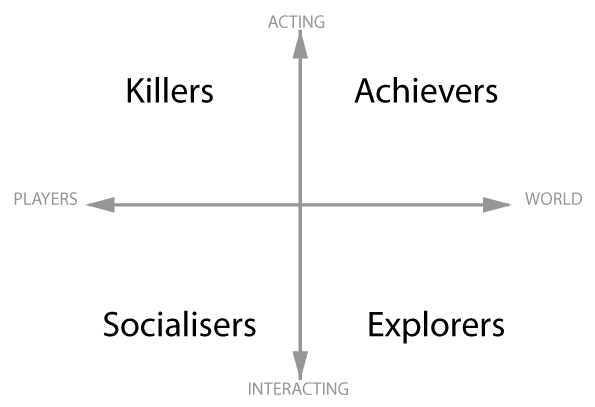
\includegraphics[scale=0.3]{figure/bartle.png}
    \caption{Bartle's taxonomy graph (adapted from \cite{bartle1996hearts}).}
    \label{fig:bartle}
\end{figure}
As it is clear in figure \ref{fig:bartle}, players that are of the Killer type will prefer games where actions involve other players, or NPCs (Non-Player Characters), while Achievers would prefer acting on the world and the environment. Socialisers and Explorer will favour interactions with other players or with the world, for example solving quests.
Even though it seems to be the most used model in game designing and game analysis, it does not seem to suit our purposes. This taxonomy fits the role playing scenario, but not the classical board games one. 
Agreeing with Bartle himself: it is not always the right tool for the job\cite{bartleyoutube}.
\subsection{Stewart's Unified Model}
In his article, Stewart analyzes a few different models -together with Bartle's- and matches all of them into a unified model\cite{stewart2011personality}. This shows how similar those models are, and that they could be almost interchangeable.
Since Bartle's model has been excluded from the list of the ones that are suitable for this project, the ones mentioned in Stewart's article have been excluded too. However, a brief description of Keirsey's model will be given further on in the chapter, as it will be useful for this thesis as a middle step for models adaptation.
\begin{figure}[H]
    \centering 
    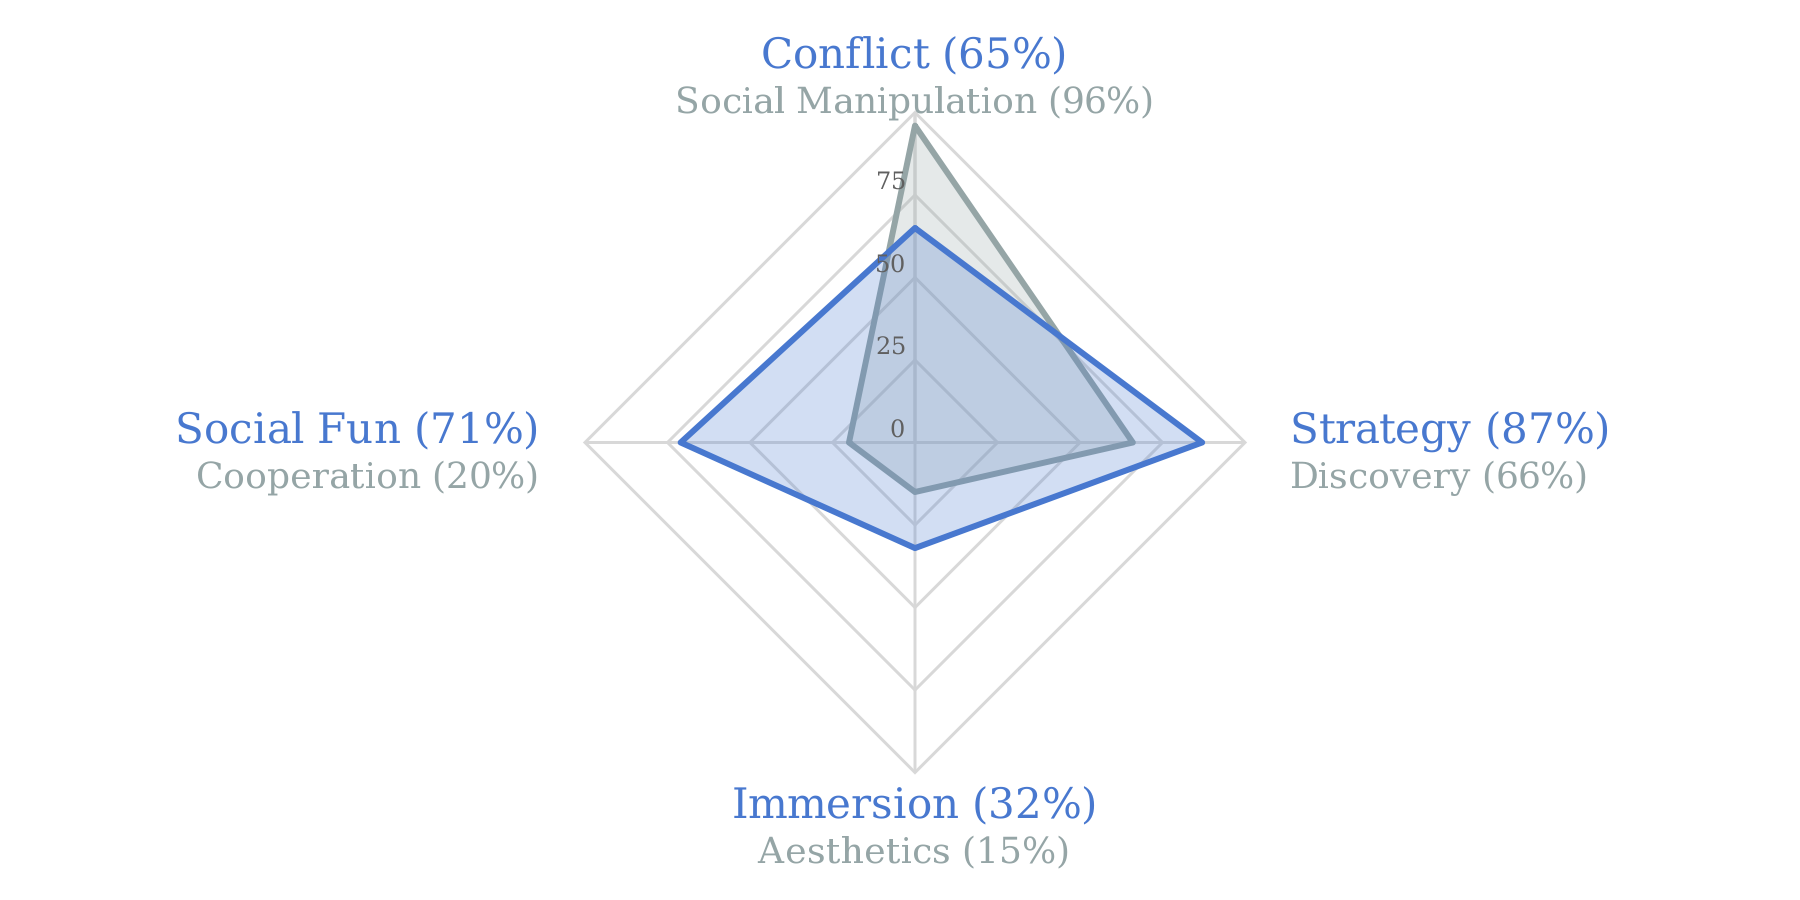
\includegraphics[scale=0.2]{figure/quanticfoundry.png}
    \caption{Example of Board Game Motivation Profile from Quantic Foundry\cite{chartprofile}.}
    \label{fig:quantic}
\end{figure}
\subsection{Quantic Foundry}
Quantic Foundry is a consulting company that works around psychology of gaming. They developed the Quantic Lab\cite{quanticfoundry}, which is a survey project aimed at understanding gamers preferences. They developed tools to test which gaming motivations are behind every player, and on their website there are two tests available, one for "Gamer Motivation Profile"\cite{yee2016gamer} and one for "Board Gamer Motivation Profile". As the first one is focused on videogames, it is outside of our scope.\\
In figure \ref{fig:quantic} can be seen an example of what are the results of the test. The profile gives a percentile rank across various motivations, as Conflict, Social Fun, Immersion and Strategy -and only secondly across Social Manipulation, Discovery, Aesthetics and Cooperation.
Even though the model seems to be pretty well-defined, it seems too complicated for this thesis' goal. It probably would be more appropriate if a bigger amount of data to work on would be available, so to force preferences over different types of games over the agent (i.e. the player that prefers immersive settings would not focus as well on classic board games, playing more sloppily that he would do if playing other games). Until the data is big enough, though, we prefer a simpler model.
\subsection{The Cardboard Republic Archetypes}
The Cardboard Republic is a website that collects board games news. They also have developed their own personality model, which consists of 6 different archetypes: Tactician, Socializer, Immersionist, Daredevil, Architect and Striker\cite{cardboard}. Their idea is to give an overview about those types, and suggest games that could be liked by the different personalities. There is a quiz on their website\cite{cardboardquiz}, and the model suggested here - based on gaming styles - seems to be highly appreciated among board gamers\cite{boardgamegeek}. 
\begin{figure}[ht]
    \centering
    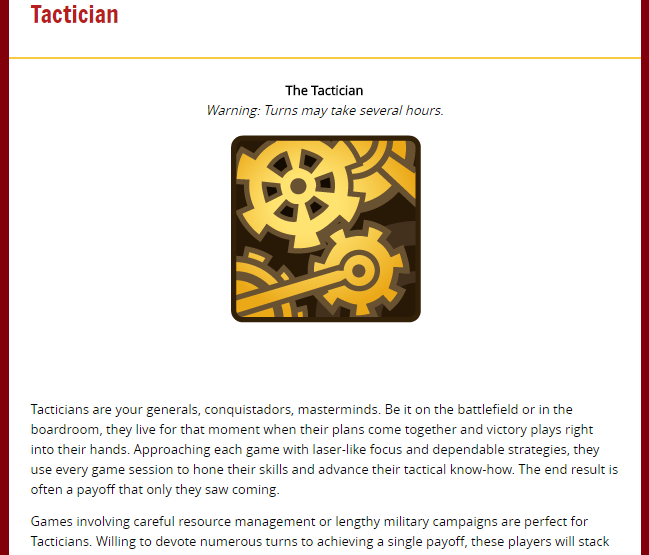
\includegraphics[scale=0.7]{figure/cardboard.png}
    \caption{Example of one of the Cardboard Republic Archetypes (from \cite{cardboard}).}
    \label{fig:cardb}
\end{figure}
In figure \ref{fig:cardb} is part of the description of the Tactician archetype, to give an idea about how the the different personalities are defined.
However, no academic resource about those archetypes has been found, limiting the credibility of being a valuable tool to use.
\subsection{Timmy, Johnny and Spike}
Timmy, Johnny and Spike are three different gamers personalities defined by Mark Rosewater and the "Magic: The Gathering" designers. It describes the three main different people that can be found while playing Magic.
Timmy defines the player who plays to enjoy "big" wins, Johnny is the player that prefers to win using hidden or peculiar strategies, and Spike is the competitive type that plays to win at all costs\cite{rosewater2002timmy}.\\
Even though this model would be simplistic enough to be used for this thesis, it feels like its is too tied to the "Magic: the Gathering" game, as it can be perceived even more in the "revisited" version of the same model\cite{rosewater2006timmy}, where the finer distinctions are based on the different behaviours of the players depending on the deck they are playing with.
It had been used as a personality model for other games, like Dominion\cite{gold2011trigram}, reaching the same conclusion about this model being game-dependent.
\subsection{BrainHex}
BrainHex is the tool developed by International Hobo Ltd to help categorize gamers while running a survey on their preferences.
They associate personalities with the parts of the brain responding to games in the specific classes, as can be seen in figure \ref{fig:brainhex}. 
\begin{figure}[ht]
    \centering
    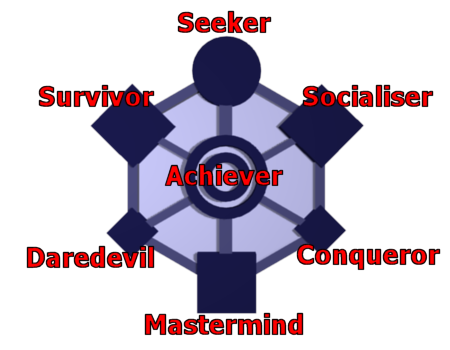
\includegraphics[scale=0.3]{figure/BrainHex_Classes.png}
    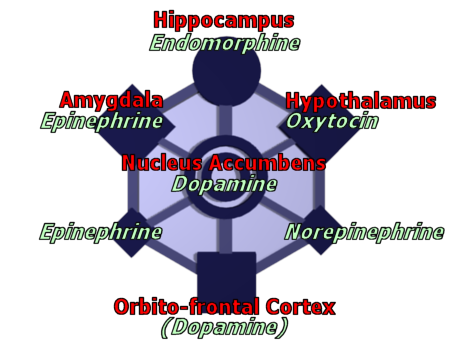
\includegraphics[scale=0.3]{figure/BrainHex_Brain.png}
    \captionsetup{justification=centering}
    \caption{On the left, BrainHex classes, on the right the corresponding parts of the brain (red text) and chemicals (green text) involved. Figure from \cite{nacke2011brainhex}.}
    \label{fig:brainhex}
\end{figure}
The personalities remind of the archetypes in the Cardboard Republic, and even though it has a more scientific background -results of a survey can be found in the article \cite{nacke2011brainhex}-, has the same complexity problem as some models described above.
\subsection{Big Five Personality Traits}\label{subsubsec:big5}
The Big Five Traits is a model widely used in psychology\cite{goldberg1993structure}, and it analyzes how personalities fall into five different scales: Openness, Conscientiousness, Extraversion, Agreeableness and Neuroticism. Each personality corresponds to a combination of the factors, helping the comprehension of behaviours and social interactions.\\
The five factors are describes as:
\begin{itemize}
\item \underline{Openness} (to experience): general openness towards emotions, new ideas, and non-ordinary situations. Low scores would imply favouring routines, and more traditional approaches.
\item \underline{Conscientiousness}: high self-discipline, sense of duty, aim for achievement. Lower scores describe careless behaviour, spontaneity, and impulsive reactions.
\item \underline{Extraversion}: higher scores imply talkativeness, sociability, and tendency to seek company of others. Lower scores describe reservedness and introversion. 
\item \underline{Agreeableness}: people with high scores are usually kind, trusting, trustworthy and considerate. Lower values imply skepticism, uncooperativeness and suspicion.
\item \underline{Neuroticism}: also called emotional instability, describe the tendency to experience negative emotions and be vulnerable to stress. 
\end{itemize}
Different scores in the factors match up in a range of various traits, giving a overall better fitting description of different personality.\cite{durupinar2008creating}\\
Unfortunately, it is not really suitable for this project, as all the factors matter equally and it would become too complicated to match users and gameplay behaviours to specific combinations. However, this was the model adopted by the project this thesis is being based on, therefore an adaption to this model was needed in order to have some continuity. A better understanding of this adaption will be given in subsection \ref{subsec:fourvsfive}. 
\subsection{Galen-Hippocrates' Four Temperaments}\label{sec:hippocrates}
Dating back to Hippocrates and Plato, the four temperaments might be one of the oldest personality models in psychology. It divides in four different categories: Sanguine, Melancholic, Phlegmatic, and Choleric\cite{merenda1987toward}. 
Shortly, the sanguine type is described as easily bored, somehow careless and as a risk-taker. Phlegmatic people are told to be diplomatic and to avoid conflicts. Cholerics are analytical, logical and goal-oriented. Melancholics are traditional and extremely ordered and accurate.
Even though there is a difference between temperaments and personality (the first one refers to innate behaviour, while the latter is built on top of the temperament, i.e. through experiences), we use the two terms interchangeably here, as what we are looking for is a simplistic model to categorize our players' behaviours.\\
Using the descriptions of each type as a guideline, and associating the model to the time responses for each type, as analyzed in \cite{chiappelli2005evidence}, those archetypes are manipulated a little, to get the results shown in table \ref{tab:temperaments} describing the playing style of each type. 
\begin{table}[ht]
    \centering
	\caption{Associated gaming skills to each of the four temperaments, in a scale from 1 to 4, where 1 means it is a strong suit for the type.}
    \scriptsize
    \begin{tabular}{|r|c|c|c|c|}
    	\hline
                        & Sanguine & Choleric & Melancholic & Phlegmatic  \\
        \hline
        Competitiveness & 3        & 1        & 2           & 4           \\
        Strategy        & 4        & 2        & 1           & 3           \\
        Analysis Paralysis      & 4        & 3        & 2           & 1           \\
        Contrasts       & 1        & 2        & 3           & 4           \\
        \hline
    \end{tabular}
    \label{tab:temperaments}
\end{table}
In table \ref{tab:temperaments} are shown the "specifics" for each personality type. A set of suits has been scaled from 1 to 4 depending on how fitting it is to each personality, where the suits are competitiveness, strategy, analysis paralysis and contrast, and they will be better described later. The scale system is applied instead of just pointing out if they are descriptive of the archetype or not in a binary fashion, in consideration of this not being exact, because of people showing different traits even if labeled with the same personality type. The table has the purpose not to strictly define a player type, but more to give an idea to our human players on what is to be expected from each temperament.
\begin{itemize}
    \item Competitiveness: shows how much a player cares about winning. It can be assumed that player types with a high value of competitiveness would do anything in order to win, without caring about how other players could perceive them. 
    \item Strategy: indicates if a player is careless in his moves or if there is a long-term plan behind. Players scoring high in strategy might play unintuitive or non-obvious moves, in order to satisfy the long-term plan. The lack of it might end up with more of short-term game (obvious moves, which give gain in the following few steps but not ultimately the best moves to win the game).
    \item Analysis Paralysis: high scores result in the player taking a long time between moves, possibly getting overwhelmed by the game and stalling.
    \item Contrast: if the player likes contrasts, it can be assumed it would play in a more aggressive and less defensive way, favouring risky moves over more conservative ones.
\end{itemize}
There are more distinctions that could be added to the table, but this already defines four very different playing styles and it feels it could be easily matched to our human players.
Unfortunately, the Phlegmatic type cannot really stand up for its skills in the games chosen in this project. A better perception of this type would be given with games that involve deception and contrast, like Werewolf\cite{werewolf} or the Resistance\cite{resistance}.
\subsection{Myer-Briggs}
The Myer-Briggs model distinguishes among 4 different bipolar traits: extroversion (E) and introversion (I), sensing (S) and intuition (N), thinking (T) and feeling (F), and judgment (J) and perception (P). It is assumed that people have a preference towards either ends of the scale, for each of those pairs, distinguishing then 16 different types of people\cite{myers2010gifts,myerbriggs}.\\ 
This model has being widely adopted in the business sector, although it is not considered as fully effective and reliable\cite{pittenger1993measuring,boyle1995myers}.
We have never considered this model as suitable for our purposes -having a too broad variety of classifications-, but since it is widely used in other contexts, we could find an adaptation between it and Keirsey's types\cite[p.~23]{keirsey1998please}.
\subsection{Keirsey's Temperaments}
Keirsey distinguishes between two basic human behaviours: communication and action. The first one could be further divided in either abstract or concrete, while actions could be defined as utilitarian or cooperative. The combination of those 4 traits forms the temperaments, which would be Artisans (concrete utilitarians), Guardians (concrete cooperators), Idealists (abstract cooperators), and Rationals (abstract utilitarians)\cite{keirsey1998please}.\\
Those four types can be further distinguished in 4 sub-types each, for a total of 16 different personalities that can be matched one-to-one to the Myer-Briggs' ones, as can be seen in table \ref{tab:keirsey-myers}.
\begin{table}[ht]
	\centering
    \scriptsize
	\caption{Keirsey's types and associated Myer-Brigg's types.}
    \begin{tabular}{|c|c|c|c|c|}
    	\hline
        Guardian & Artisan & Idealist & Rational\\
        \hline
        Supervisor & Promoter & Teacher & Fieldmarshal\\
        (ESTJ) & (ESTP) & (ENFJ) & (ENTJ)\\
        \hline
         Inspector & Crafter & Counselor & Mastermind\\
         (ISTJ) & (ISTP) & (INFJ) & (INTJ)\\
         \hline
         Provider & Performer & Champion & Inventor\\
         (ESFJ) & (ESFP) & (ENFP) & (ENTP)\\
         \hline
         Protector & Composer & Healer & Architect\\
         (ISFJ) & (ISFP) & (INFP) & (INTP)\\
		\hline
    \end{tabular}
    \label{tab:keirsey-myers}
\end{table}
This model was described in Steward's unified model\cite{stewart2011personality}, and being proposed as interchangeable with Bartle's taxonomy, not taken into consideration as base model for the project.\\
\section{General Game Playing}\label{sec:ggp}
Games have been found suitable for the development of Artificial Intelligence for many years now; in \cite{schaeffer2002games}, Schaeffer and van Der Herik present an interesting overview on the topic. In this project, we will focus on the branch called General Game Playing (GGP), firstly described by Pell's thesis\cite{pell1993strategy}. General Game Playing deals with agents learning new games without prior knowledge or ad-hoc strategy. The rules are given to the player only once the game has started, and the agent will have to work out a strategy while the match is ongoing. Contrarily to gaming agents like Deep Blue\cite{campbella2002deep} or AlphaGo\cite{silver2016alphago}, a General Game Player is not supposed to know a-priori any game-specific heuristic, and the heuristics it is supposed to be supplied with need to be applicable to any game, hence the word General. The subject includes a broad range of topics in AI, as knowledge representation, search algorithms, machine learning and, of course, game playing\cite{genesereth2014general}.
\subsection{Games Structure}
Innumerable games could be proposed to General Game Players, as long as they satisfy the common requirements: the games are supposed to have a fixed number of players, and can be defined as in definition \ref{def:game}.\\
\begin{definition}\label{def:game}
A game in GGP can be described as an automaton defined by a tuple ${<S,A,\delta,s_0,\Gamma, G_p>}$, where:
\begin{itemize}
\item ${S}$ is a finite number of states;
\item ${A}$ is a finite set of actions;
\item ${\delta}$ is the transition function, where ${\delta: S \times A \rightarrow S}$;
\item ${s_0}$ is the initial state, where ${s_0 \in S}$;
\item ${\Gamma}$ is the set of final states, where ${\Gamma \subseteq S}$;
\item ${G_p}$, the goal function associated to each player ${p}$, for each state $s \in S$.
\end{itemize}
\end{definition}
Only a subset of the games available for General Game Playing will be considered here: all of them are perfect information games, turn-dependent, and bounded to 2 players, as will be further described in section \ref{subsec:rulesgames}.
Games are represented with state machines (see appendix \ref{app:prel} for further information), specifically, they can be seen as trees, where each node-successor represents the legal moves from the parental node. Additionally, games are also Markov Decision Processes\cite{bellman1957markovian} -better described in \ref{sec:ml}-, as the history of transitions between states is irrelevant in the decision process for the future, at any given point\cite[p.~189]{genesereth2014general}.\\
When the game starts, the players are provided with the rules of the games, described in Game Description Language (GDL)\cite{love2008general} -a logic language, variant of Prolog. The language has recently been extended (GDL-II) to allow description of imperfect information games\cite{thielscher2010general,schiffel2011reasoning}.\\
In GGP, every game must be playable and weakly winnable - if multiplayer -, or strongly winnable - if single-player -, according to definitions \ref{def:playable} and \ref{def:winnable}, as found in \cite{genesereth2005general}.\\
\begin{definition}[Playability]
\label{def:playable}
A game is playable if and only if every player has at least one legal move in every non-terminal state.
\end{definition}
\begin{definition}[Winnability]
\label{def:winnable}
A game is weakly winnable if and only if, for each player, there is a sequence of joint moves of all players that lead to a terminal state where that player's goal is maximal. A game is strongly winnable if and only if, for some players, there is a sequence of individual moves that leads to a terminal state of the game where that player's goal value is maximal.
\end{definition}
The administration of the matches is left to the Game Manager, which communicates to and with the players regarding the ongoing game, i.e. informing when the respective turns start -passing over the state of the board and the list of previous actions-, or when the game is over. In figure \ref{fig:GGP} we can see the idea behind a GGP system\cite{genesereth2014general}.\\
\begin{figure}[H]
\centering
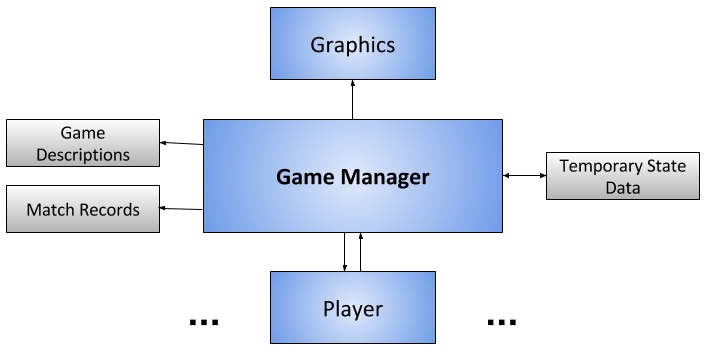
\includegraphics[scale=0.4]{figure/GGP2}
\caption{Diagram of a classical GGP environment (adapted from \cite{genesereth2014general}).}
\label{fig:GGP}
\end{figure}
The player used for this project uses a Monte Carlo Tree Search algorithm to find a strategy, and has been modified to go through already played games, and it will be further described in section 3.2.\\
\section{Monte Carlo Tree Search Algorithm}\label{sec:mctstheory}
Monte Carlo Tree Search has become more and more popular recently, due to the simplicity of implementation and the generality of application. It has been applied to a multitude of scenarios, giving satisfying results. Sticking to the games' development in the field of artificial intelligence, the Monte Carlo Tree Search algorithm has been applied to a variety of games: Go\cite{gelly2011monte,gelly2006modification,enzenberger2010fuego}, Hearts\cite{santoevaluating}, Settlers of Catan\cite{szita2009monte}, Amazons\cite{lorentz2008amazons}, and Lines of Action\cite{winands2010monte,winands2009evaluation} among the others. Moreover, it can also be associated with the best players participating in the General Video Game Playing Competition\cite{perez20162014}.
\\The algorithm has been developed starting from the idea of Monte Carlo methods, which obtain results relying on random sampling. In the search case, the Monte Carlo sampling is associated to a tree structure, where - when applied to games - each node represents a state in the game, and contains the current QValue and a value $n$, where $n$ is the number of visits for that specific state\cite{chaslot2008progressive}. The algorithm could be summarised in four main steps\cite{chaslot2010monte}, as can also be seen in \ref{fig:mcts}: 
\begin{enumerate}
\item \emph{Selection}: starting from root, and until a terminal node is hit, a leaf child node is recursively selected for expansion;
\item \emph{Expansion}: children nodes are added to the tree, depending on the available moves in the current state;
\item \emph{Simulation}: one play-out is run through until a value \emph{chargeDepth} limit is reached. A parameter \emph{epsilon} decides whether a random move is picked, or if MAST (Move-Average Sampling Technique, better described in the next paragraph) is applied.
\item \emph{Backpropagation}: the nodes in the tree get updated with the results from the simulation, associating a value $Q(s,a)$ to each node, defined as \begin{equation}\label{eq:mcts}
Q(s,a) = \frac{1}{N(s,a)} \sum_{i=1}^{N(s)} \chi_{i}(s,a) z_i
\end{equation}
where, using the same notation as \cite{gelly2011monte} and \cite{browne2012survey}, $N(s,a)$ is the number of times action $a$ has been simulated from state $s$, $N(s)$ describes how many times a game has been played out through state $s$, $z_i$ is the result of the $i$th simulation played out from $s$, and\\ $$\chi_{i}(s,a) = 
\begin{cases}
1 & \text{if }a\text{ was selected from state }s\text{ during $ith$ playout};\\
0 & \text{otherwise}.
\end{cases}$$
\end{enumerate}
\begin{figure}[ht]
    \centering 
    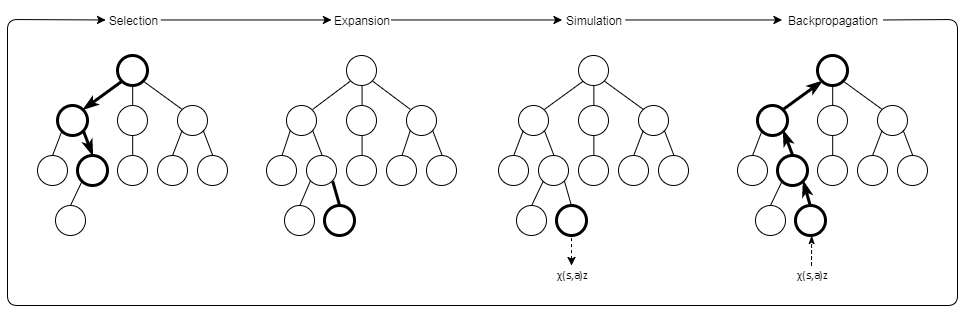
\includegraphics[scale=0.4]{figure/MCTS.png}
    \caption{Iteration of MCTS (graph adapted from \cite{browne2012survey,chaslot2008progressive,winands2010monte}).}
    \label{fig:mcts}
\end{figure}
In the case of this project, the search ends when \emph{Limit} simulations - set as a constant $limit = 1000$ - is reached, but could be replaced by any time or memory constraints. 
\subsection{Monte Carlo Tree Search Enhancements}
The search can be associated to a set of other algorithms and tree policies, that can lead to quicker results compared to the basic Monte Carlo Tree Search, and might be preferred in some particular circumstances. In \cite{browne2012survey} we can find a comprehensive survey of the Monte Carlo Tree Search methods that have been implemented so far, and we would like to refer to it if the reader is interested in further information. Different enhancements can be applied at different stages of the search, it is then possible - and suggested - to apply multiple algorithm at once\cite{finnsson2010learning}; in our case, our algorithm uses UCT with RAVE and GRAVE as extensions for the learning process, and MAST as a search-control policy, and they will be better described later in this chapter. First thing, though, it is necessary to define what bandit problems are.
\subsubsection*{Bandit problems and Upper Confidence Bound (UCB)}
Bandit problems are a class of sequential decision problems that could be modeled over slot machines (known as "one-armed bandit" in Las Vegas), and describes the \emph{exploitation-exploration dilemma}, which is the problem of finding equilibrium between exploiting an action that appears to be optimal in the short run, and exploring the search space for a temporarily less-optimal but overall better one. Assuming to be in a room with $K$ slot machines, while having no knowledge of the past observations, our goal is to collect information about each slot machine by pulling their levers, while maximizing our cumulative reward at the same time. A K-armed bandit can then be described as a set of random variables $X_{i,n}$, with $1\leq i \leq K$ and $n\geq1$, and where $X_{i, n}$ represents the reward of pulling arm $i$ for the $n$th time. All $X_{i,n}$ are independent and identically distributed for all $n$, accordingly to an unknown distribution, with unknown mean $\mu_i$. Which bandit to play is decided with the aid of a \emph{policy}, whose goal is to minimize the regret of the player, defined as $\nu_n = \mu^*n-\mu_i \sum_{i=1}^{K}\mathbb{E}[T_i(n)]$, where $\mathbb{E}T_i(n)$ is the expected number of plays of arm $i$ in the first $n$ tries, and $\mu^*$ is the best possible reward\cite{browne2012survey,auer2002finite,kocsis2006bandit,kocsis2006improved,shivaswamy2012multi}. It is known that the slowest growing regret policy is $O(\ln n)$, as described by Lai and Robbins in \cite{lai1985asymptotically}, and one the simplest applicable policies, with expected logarithmic growth, is \emph{Upper Confidence Bound (UCB)}, first published by Auer et al. \cite{auer2002finite}, and defined as $$UCB1 = \overline{X}_i + \sqrt[]{\frac{2\ln n}{n_i}}.$$
\subsubsection*{Upper Confidence Bounds for Trees (UCT)}
Firstly proposed by Kocsis and Szepesvári \cite{kocsis2006bandit,kocsis2006improved}, UCT considers every state in the game as a multi-armed bandit problem, taking advantage of \emph{UCB1} and its simplicity and efficiency for the children selection. Then, the selection of child node $i$ depends on maximizing $$UCT = \frac{w_i}{n_i}+C_p*\sqrt[]{\frac{\ln N}{n_i}}$$ where $w_i$ is the number of wins after move $i$, $n_i$ is the number of simulations for move $i$, $N$ is the total number of simulations for the current node, and $C_p$ is a constant that we will be passing as a parameter called $ExplorationFactor$.
\subsubsection*{Rapid Action Value Estimation (RAVE)}
RAVE is part of policies that correspond to the name of \emph{All Moves As First} (AMAF)\cite{brugmann1993monte,helmbold2009all}. In this case, it is combined with UCT, as first done by Gelly and Silver\cite{gelly2007combining,gelly2011monte}, and it is meant to speed up the nodes' values evaluation, updating the value of each action every time it is taken, even in subsequent courses of action, and not only when it is specifically selected at one state. RAVE is based on a class of AMAF algorithms called $\alpha$-AMAF, which calculates the score for each action as $$\alpha Q_a+(1-\alpha)U$$ where $U$ is the UCT score, and $Q_a$ is the Q value for action $a$. In the RAVE case, we have a parameter $\beta$ instead of $\alpha$, which is calculated as $$\beta=\sqrt[]{\frac{Rave}{3*n+Rave}}$$ where $n$ is how many times the node has been selected, and $Rave$ is the value passed as parameter to our search, representing the number of visits a node can have before RAVE is not used anymore\cite{browne2012survey,gelly2007combining,gelly2011monte}.
\subsubsection*{General Rapid Action Value Estimation (GRAVE)}
GRAVE can be considered a generalization of RAVE, where a node is considered to have reliable statistics only when a certain number of playouts has been carried out. This value is passed as parameter $Grave$, and when the number of playouts is grater than it, then the values of the actions are calculated using general RAVE, otherwise the closest parent with a satisfying number of playouts is used as a reference to calculate the value for $Q_a$\cite{cazenave2015generalized}. 
\subsubsection*{Move Action Sampling Technique (MAST)}
The MAST method has firstly been described in \cite{finnsson2008simulation} and applied in CADIAPLAYER \cite{finnsson2007cadia}. This technique keeps track of the average value of each move, updated at backpropagation, and independent from the state it has been played in. From literature, it is known that, on the long run, actions $a$ with an higher average value $Q_{mast}(a)$ are most likely to be better than the ones with lower average\cite{finnsson2009simulation}. During playout the move selection can then be biased, with probability distribution corresponding to Gibbs distribution, as $$P(a) = \frac{e^{Q_{mast}(a)/\tau}}{\sum_{b=1}^n e^{Q_{mast}(b)/\tau}}$$ where $\tau$ is a parameter that controls the distribution, and $Q(a) = max GGP score = 100$, if $a$ hasn't been explored yet\cite{finnsson2008simulation,finnsson2007cadia,finnsson2009simulation}.
\subsubsection*{Discounting}
Two different discounts are applied to the moves values, controlled by two separate variables. One discount, depending on a variable called $ChargeDiscount$, applied at backpropagation, and the second discount, depending on $TreeDiscount$, is applied as a discount in the tree. It is thought that the search tree results are more reliable than the ones found at charge, therefore only a smaller discounting needs to be applied\cite{helgadottir2016virtual}.
\subsubsection*{Early Cut-Off}
Running Monte Carlo Tree Search algorithms might be time consuming, so a limit can be introduced to try to skim the moves that look more unappealing, so to focus better on the moves that are more promising\cite{finnsson2012generalized}. A limit $ChargeDepth$ is applied to the tree size, in order to make sure that a response to the opponent is being sent back in a decent amount of time. When this limit is hit by our search, a set of default values is returned, controlled by an array of variables called $ChargeDefaults$, one for each player\cite{helgadottir2016virtual}.
\subsubsection*{Heuristics}
Innumerable heuristics could be applied, either game-dependent (i.e. through piece counting\cite{helgadottir2016virtual}), based on the move selection history\cite{schaeffer1989history}, or used as personality bias. The latter is the case applied in this project's search, with two arrays of variables - one per each player - called $Aggressiveness$ and $Defensiveness$, and one value called $NiceThreshold$. As the names are mostly self-explicable, $Aggressiveness$ and $Defensiveness$ are controlling the goals of the game, being an increasing or decreasing factor, depending on the current state of the game. Considering that the maximum goal is $100$, and the minimum is $0$, we have that:
\begin{itemize}
\item If $goal_{current}>85$, the game can be considered as already won, and no biases are applied;
\item if $60<goal_{current}<85$, then the goal is biased using the $Aggressiveness$ value;
\item if $goal_{current}<35$, then the goal is biased using the $Defensiveness$ value;
\item if $35 \leq goal_{current} \leq 60$, then a value $r$ is picked uniformly at random in $[0,1]$ used to select with probability $P_{a,d}=0.5$ which bias to apply, $Aggressiveness$ or $Defensiveness$.
\end{itemize}
It is to be noted that $goal_{current}$ takes its value from the games rule, and most games only expect a win, a loss, or a draw, corresponding to 100, 0, or 50 points each. The values get then discounted, allowing to have some more flexibility with the $goal_{current}$ values described above.\\
Lastly, the value $NiceThreshold$ controls which difference in goals sets the AI to lower its standards and pick a sub-optimal move instead of the best one, to make the gaming experience more enjoyable for the opponent\cite{helgadottir2016virtual}.\\
Although those parameters have relatively less influence in the search outcome itself, it is easier to intuitively relate them to specific personality types. For example, looking back at table \ref{tab:temperaments}, a higher $Aggressiveness$ value would be expected for higher "Contrasts", hence for Sanguine users, as well as lower $NiceThreshold$ for more competitive players, as Choleric and Melancholic people are supposed to be.\\
\section{Machine Learning}\label{sec:ml}
Machine learning refers to the concept of extrapolating patterns and information from data. There are three main learning approaches that are applied in machine learning: supervised learning, where the agent learns to map certain outputs depending on specific inputs; unsupervised learning, where the agent is given an input and is meant to discover patterns in the outputs, so to be able to draw any conclusion about the data; and lastly, reinforcement learning, where behaviour is meant to be learnt depending on rewards or punishments. In the case of unknown reward functions that need to be withdrawn from observed behaviour, the problem becomes an inverse reinforcement learning one. In the case of this thesis, the problem falls in the supervised learning field. Classical methods for supervised learning could not be applied in this project, due to the complexity of the model used.
In this section will be defined the information needed to understand the Bayesian probability model in section \ref{sec:mlmethod}. A Bayesian approach simply means calculating each hypothesis' probability and using them to infer predictions from the data\cite{russell1995modern}.\\ The combination of a Bayesian framework and excerpting of preferences has gotten promising results in literature\cite{rothkopf2011preference}, as well the combination of Bayesian statistics and evolutionary algorithms, as for example in \cite{turner2012375}, where an Approximate Bayesian Computation algorithm (ABC) has been combined with a Differential Evolution one, in \cite{pelikan2003hierarchical}, where Bayesian Networks were used instead, or in \cite{wawrzynczak2014data}, where Bayesian Inference has been matched with Genetic Algorithms. 
\subsection{Decision Theory and Preference Elicitation}
Looking at the games' structure, it is easy to associate the problem of selecting the next move in a game to the topic of Decision Theory, which is an interdisciplinary field intuitively defined as the analysis of choices between options, each one having an expected utility value. The underlying idea in decision theory is called Maximum Expected Utility (MEU), where \emph{"an agent is rational if and only if it chooses the action that yields the highest expected utility, averaged over all the possible outcomes of the action"}\cite{russell1995modern}. In the specific, not having a full picture of the actions choices for all states of each game, the problem tried to be solved in this thesis falls in the class of "Decision Making Under Uncertainty", which, as the name hints, refers to the problems where either information or knowledge are incomplete\cite[p.~3-4]{scholz1983decision}. Even more specifically, the goal to extract preferences depending on the personality of the player would fit in the Preference Elicitation problem, as it tries to identify the favourite events of a group of people, over the set of available actions that can be selected from being in a certain state, depending on the group's personality. The choices throughout games are here extracted from a Monte Carlo Tree Search algorithm, described previously, which has a set of controlling parameters the actions picked depend on. Different sets of parameters lead to different actions, hence the decisions should be able to be associated to a set of MCTS parameters. This set is meant to be found using a Genetic Algorithm -described later in this chapter-, with a fitness function that represents the expected utility function mentioned earlier.
Our hypothesis is assuming multiple major differentiation of people's behaviour in game playing, based on specific personalities. We are expecting that games played by people with different personality would develop with different types of underlying strategies, than if compared to people with the same personality. The implementation of our algorithm is foreseeing the application of a diverse set of parameters, depending on the personality of the player.\\
\subsection{Markov Decision Process}
It has been mentioned in \ref{sec:ggp} that the games in General Game Playing are seen as Markov Decision Processes. In order to clarify what a Markov Decision Process is, it is necessary to start defining the Markov property. Let $I$ be a state-space, $X$ is a random variable with values in $I$ where $X:\Omega\rightarrow I$, then $$\lambda_i=\mathbb{P}(X=i)=\mathbb{P}({\omega : X(\omega)=i}).$$
It is said that $(X_n)_{n\geq 0}$ is a Markov chain with initial distribution $\lambda$ and transition matrix $H=(h_{ij}:i,j \in I)$ if
 \renewcommand{\labelenumi}{(\roman{enumi})}
\begin{enumerate}
\item $X_0$ has distribution $\lambda$;
\item for $n\geq 0$, conditional on $X_n=i$, $X_{n+1}$ has distribution $(h_{ij}:j\in I)$ and is independent of $X_0,\cdots X_{n-1}$.
\end{enumerate}
\begin{theorem}
A discrete-time random process $X_{n_{0\leq n \leq M}}$ is a Markov chain ($\lambda$,H) (or just called Markov($\lambda$,H)) if and only if $\forall i\ i_1,\cdots,i_N\in I$ $$\mathbb{P}(X_0=i_1, X_1=i_2,\cdots,X_N=i_N)=\lambda_{i_1}h{i_1i_2}h{i_2i_2}\cdots h{i_{N-1}i_N}.$$ 
\end{theorem}
Additionally:
\begin{theorem}
Let $(X_n)_{n\geq 0}$ be Markov$(\lambda,H)$. Then, conditional on $X_m=i$, \\$(X_{m+n})_{n\geq 0}$ is Markov$(\delta_i,H)$ and is independent of the random variables $X_0,\cdots,X_m$.
\end{theorem}
The proofs are let to be read in \cite{norris1998markov}, where we have taken the cue from for the above theorems and definitions. However, more informally speaking, the Markov property is assuming that the Markov Chain $X$ is in a current state $s_t$, then no additional information is given by how $s_t$ has been reached. Therefore, the current state $s_t$ provides enough information for the reward to be computed without looking at previous states. Subsequently, Markov Decision Process can then be defined as sequential decision processes with a Markovian transition function and a reward function\cite{russell1995modern}. More formally, adapting from \cite{puterman2014markov} and \cite{ng2000algorithms}:
\begin{definition}
A (finite) Markov Decision Process (MDP) is a tuple \\$<S, A, P_{sa}, G_.(\cdot,\cdot),\xi>$, where:
\begin{itemize}
\item $S$ is a finite set of states;
\item $A$ is a finite set of actions;
\item $P_{sa}(\cdot)$ are the state transition probabilities upon taking action $a$ in state $s$;
\item $G_p(s,s')$ is the reward function;
\item $\xi\in[0,1]$ is the discount factor.
\end{itemize}
\end{definition}
\section{Genetic Algorithm}\label{sec:gatheory}
The information to be inferred from the dataset is a set of parameters which can be used as input to an agent, expecting that the output actions will match humans', when the human has the same personality as the agent being trained. In order to do determine this specific set of parameters, an optimization algorithm is applied over the fitness function \ref{eq:mcts}. The approach adopted is a Genetic Algorithm.\\ Genetic Algorithms (GA) are part of the family of stochastic optimization methods, and are based on Evolutionary Algorithms, having the purpose to study the adaptation of individuals throughout time. First implemented by John Holland and his colleagues and students between 1960s and 1970s\cite{holland1992adaptation}, there has been a growing interest in the topic in the past years. Evolutionary Algorithms take their terminology from biology, being inspired by it in the first place. The concept of \emph{population} is then introduced as a set of \emph{individuals}. Each \emph{individual} has a \emph{chromosome}, formed by a set of \emph{genes}. A more detailed description of the biological terminology can be found in \cite[p.~5]{mitchell1998introduction} and in \cite[p.~35]{wahde2008biologically}, while here the vocabulary will be limited to what is strictly related to the purposes of this project.\\Genetic Algorithms are finite, however, the outputted solution might be due to premature convergence, and only be a local optima, therefore there is no complete certainty of finding the actual optimal solution. 
\subsection{General Structure}
There is no final definition of GAs, but a general structure can be drawn from literature:
\begin{itemize}
\item \emph{Individual}: a set of \emph{genes}. The \emph{genes} have a defined \emph{encoding scheme}, that can be binary encoding scheme, strings, real numbers, integers, and so on. 
\item \emph{Population}: a family of $\Psi$ individuals is initialized at random, forming the first \emph{generation} of the population.
\item \emph{Fitness function}: is a function $F$ whose value is calculated at evaluation time. The overall goal of optimization problems is to maximise (or minimise) the value of this function.
\item \emph{Evaluation}: each \emph{individual} $i$ is evaluated, after being decoded in the relative variable, and the value of $F(i)$ is calculated, where $F$ is the \emph{fitness function}, and $i=1,...,\Psi$.
\item \emph{Selection}: in order to form the next \emph{generation} it is needed to select which \emph{individuals} will survive evolution, and which will not. There are multiple strategies for selection, where the more popular are tournament selection, roulette-wheel selection and ranking selection. Those methods will be further described in subsection \ref{subsec:selection}.
\item \emph{Elitism}: keeping track of our best individual generation after generation reduces the risk of having a decreasing fitness due to mutation or crossover. It has been shown that combining elitism to a selection algorithm improves the final results\cite{baluja1995removing}.
\item \emph{Crossover}: the reproduction of the individuals happens through a crossover algorithm, where, once two parents are picked, two new individuals containing genes from either parents are added to the next generation. Further information about the topic can be found in subsection \ref{subsec:cross}.
\item \emph{Mutation}: Once the new generation is born, a mutation can happen to none, one or multiple genes in each individual. A description of how mutation happens over this project's encoding can be found in \ref{subsec:mut}.
\end{itemize}
\subsection{Selection}\label{subsec:selection}
In this section, three different algorithms for the selection process will be described. Only the roulette-wheel selection has been used in this thesis, as specified in \ref{sec:ga}, but the other two algorithms have been considered and might have been applied for comparison if there were no time constraints.\\
\textbf{Tournament selection}\qquad
Tournament selection, as the name hints, it is the selection process carried out as a tournament. Once defined a tournament size $t_s$, $t_s$ individuals are taken and compete for survival. The lower $t_s$ is, the higher the competition. This flexibility makes this approach one of the most widely used in GAs\cite{miller1995genetic}.\\
\textbf{Roulette-wheel selection}\qquad
The roulette-wheel strategy selects individuals proportionally to their fitness value. To obtain the resemblance with an actual roulette-wheel, a cumulative fitness function is calculated as $$\phi_j=\frac{\sum^i_{j=1} F(j)}{\sum^\Psi_{i=1} F(i)},\hfill j=1,...,\Psi$$ where $F(i)$ is the fitness value of individual $i$. A value $r$ is drawn uniformly at random in $[0,1]$, and the individual with the smallest $j$ that satisfies $r<\phi_j$ is selected\cite{wahde2008biologically}. \\
\textbf{Rank selection}\qquad
Firstly defined in \cite{baker1985adaptive}, it ranks all the individuals depending on the value of their fitness function, from rank $\Psi$ for the best individual, to $1$ for the worst. Each individual $i$ has then an associated probability of being selected, calculated as $$P(i)=\frac{1}{\Psi}\big(\eta^-+(\eta^+-\eta^-)\frac{i-1}{\Psi-1}\big);\hfill i\in{1,...,\Psi}$$ where the conditions $\eta^+=2-\eta^-$ and $\eta^-\geq0$ are satisfied, since the population size is constant, and $\frac{\eta^-}{\Psi}$ is the probability of selecting the worst individual in this generation's population, while $\frac{\eta^+}{\Psi}$ is the probability of selecting the fittest\cite{blickle1995comparison}.
\subsection{Crossover}\label{subsec:cross}
Here, the most used crossover algorithms will be described; the first, because we think it helps to have a better understanding of the crossover process, and a second one, which is the algorithm that has applied in this project. Further techniques can be found in \cite{umbarkar2015crossover}.\\
\textbf{Single Point Crossover}\qquad
A popular way of applying crossover is to decide on a "barrier" $c$, and create the offspring $o_1$ and $o_2$ with $c$ genes from one of the parents, and $(G-c)$ genes from the other one, where $G$ is the total number of genes in an individual. This approach is called Single Point, and it is represented in figure \ref{fig:crosssp}.
\begin{figure}[H]
    \centering 
    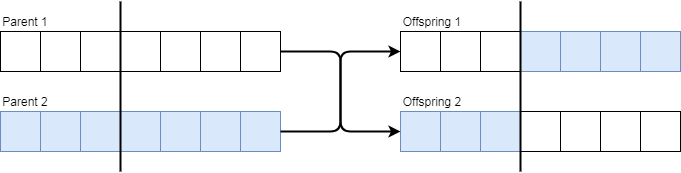
\includegraphics[scale=0.5]{figure/Crossoversinglepoint.png}
    \caption{Example of Single Point crossover between two individuals.}
    \label{fig:crosssp}
\end{figure}
Deriving from this idea, there is Two-Points crossover, as well as Multi-Points Crossover, which explanation at this point is trivial.\\
\textbf{Averaging Crossover}\qquad
Given two individuals as parents, this approach returns two children $o_1$ and $o_2$ with genes calculated as an average from the parents' $p_1$ and $p_2$, as $$g_{o_1} = \alpha g_{p_1} + (1-\alpha)g_{p_2}$$ and $$g_{o_2} = (1-\alpha) g_{p_1} + \alpha g_{p_2}$$ where $\alpha$ is chosen uniformly at random in $[0,1]$\cite{ladkany2012genetic}, for each gene $g$.
\subsection{Mutation}\label{subsec:mut}
Any gene in any individual could be subjected to mutation, depending on probability $P_{mut}$. When dealing with genes encoded with real numbers, the most common approach for mutation is the real-number creep, where a creep value limits the range of values the new gene can take. Let $C_r$ be the creep rate, then the new gene is $$g\Leftarrow g-\frac{C_r}{2}+C_r\gamma=g+C_r(\gamma-\frac{1}{2})$$ where $\gamma$ is picked uniform at random in $[0,1]$\cite[pp.~53-55]{wahde2008biologically}.
\subsection{Termination} 
GA usually stops when there is stagnancy: either the fitness function has not been increasing for generations, or the individuals converged to very similar ones (leading to a very similar fitness function too). In other cases it is preferred to give a fixed number of generations to run the GA for; in other, a decency fitness test is added, stopping the algorithm when a minimum fitness value is reached, finding an acceptable result instead of the optimal one. In this project, a stagnancy test has been adopted, and it will be further described in section \ref{sec:ga}.
